\documentclass{article}
\usepackage{graphicx, caption, subcaption, verbatim, moreverb, alltt, algorithm2e, kotex}
\usepackage[protrusion=true,expansion=true]{microtype}
\usepackage{fancyvrb}
\usepackage{hhline}
\usepackage{multirow}
\DeclareGraphicsExtensions{.pdf,.png,.jpg}
\let\verbatiminput=\verbatimtabinput

\setlength{\oddsidemargin}{0.25in}	% 1.25in left margin 
\setlength{\evensidemargin}{0.25in}	% 1.25in left margin (even pages)
\setlength{\topmargin}{0.0in}		% 1in top margin
\setlength{\textwidth}{6.0in}		% 6.0in text - 1.25in rt margin
\setlength{\textheight}{9in}		% Body ht for 1in margins
\addtolength{\topmargin}{-\headheight}	% No header, so compensate
\addtolength{\topmargin}{-\headsep}	% for header height and separation

\begin{document}

\title{Lab 6: 6-stage Pipelined Processor}   % type title between braces
\author{CSE 4190.308 Computer Architecture \\ 2 Exercises (Total 80 Points) }         
\date{Received: May 2, 2013 \\Due: 3:00 p.m., May 16, 2013\\ \ \\ TA Office Hours: 7:00 - 8:00 p.m., 5/13, 5/14, 5/15}    % type date between braces
\maketitle

\section{Introduction}

In this lab, you will be given a 2-stage pipelined processor,
and change it into a 6-stage pipelined processor.
Because all kinds of hazards covered in class will exist in a 6 stage
pipeline, it will be your job to use methods such as epochs, scoreboards and bypassing (forwarding)
correctly to implement a functionally correct
and efficient 6-state pipelined processor.

%Compiling and running the code can be done identically to the previous
%labs, using the \texttt{smips} run script.

\section{Getting Started}
\subsection{How to Download the Source Code}
Lab 6의 실습 코드를 받기 위해 수업 홈페이지에 올라와 있는 \texttt{add-lab6.sh} 스크립트를 다운받고,
이전 Lab들을 수행했던 실습 디렉터리의 상위에 위치시킨 뒤 본인의 ID를 인자로 실행시킵니다.
archi13의 passward(강의 홈페이지 비밀번호)와 본인의 svn 계정 비밀번호를 입력하면 실습 코드 다운이 완료됩니다.
실습 디렉터리 아래에 \texttt{lab6} 디렉터리가 새롭게 생성되었을 것입니다.

\begin{Verbatim}[frame=single]
   $ ./add-lab6.sh YOUR_ID

   archi13@hyewon.snu.ac.kr's password: 

   Password for 'YOUR_ID': 

   $ ls YOUR_ID/
   ... lab4/ lab5/ lab6/
\end{Verbatim}

\subsection{Directory Structure of Lab 6}
Lab 6 실습의 디렉터리 구조는 다음과 같습니다.

\begin{Verbatim}[frame=single]
lab6/
    src/	
        Proc.bsv
        smips
    lib/
        common-lib/
        compiler/
        programs/
        ...
\end{Verbatim}

\begin{description}
\item [\texttt{src/}]\hfill \ \\
	Lab 6 실습을 진행할 디렉터리입니다.

\item [\texttt{src/Proc.bsv}]\hfill \ \\
	2-stage pipeline SMIPS 프로세서가 구현되어 있는 파일입니다.

\item [\texttt{src/smips}]\hfill \ \\
	구현한 프로세서를 컴파일하고 벤치마크 프로그램을 실행할 수 있는 스크립트 파일입니다.

\item [\texttt{lib/}]\hfill \ \\
	Lab 에서 구현한 SMIPS 프로세서를 동작시키는 데 필요한 라이브러리 및 프로그램을 포함하고 있습니다.

\item [\texttt{lib/common-lib/}]\hfill \ \\
	프로세서를 구현할 때 사용되는 라이브러리 bsv 파일들입니다.

\item [\texttt{lib/compiler/}]\hfill \ \\
	C 언어로 작성된 벤치마크 프로그램을, SMIPS 프로세서에서 실행시킬 수 있도록 
	SMIPS 어셈블리 프로그램으로 변환해주는 컴파일러입니다.

\item [\texttt{lib/programs/}]\hfill \ \\ 
	구현한 프로세서를 테스트하기 위한 벤치마크 프로그램들입니다.

\end{description}

\subsection{How to Simulate the Design}
Lab 6 consists of Exercises that requires to improve and modify the given 2-stage pipeline processor.
Instead of a makefile, we have provided a script file that take care of everything. 
The \texttt{smips} script will take care of everything from compiling
the SMIPS core and cross-compiling the benchmarks for SMIPS, to running the benchmarks.

In order to compile the processor and all benchmarks and run them,
you can use the following command:

\begin{Verbatim}[frame=single]
./smips -c all -r
\end{Verbatim}

The \texttt{-c} flag specifies which benchmarks to compile, and the
\texttt{-r} flag tells the script to run the benchmarks that has been
compiled. After completing execution, the script will tell you if your
processor has passed the benchmark, and how many cycles it took to
execute how many number of instructions.

\sloppy
You can also pick individual benchmarks to compile and run, instead of
\texttt{all}. You can do this by pointing to the individual benchmark
directory. These benchmarks can be found in the directory
\texttt{lib/programs/src/}. For example, the
\texttt{multiply} benchmark can be run using the following command:

\begin{Verbatim}[frame=single]
./smips -c multiply -r
\end{Verbatim}

\sloppy
You can learn other arguments that the scripts take, by
running:

\begin{Verbatim}[frame=single]
./smips -h
\end{Verbatim}

You can also see what happened in each pipeline step of each cycles.
You will find directories named as the benchmarks in the \texttt{build} directory
after you finished running benchmark programs. The \texttt{simOut} files in these
directories contain the information on how instructions passed by each pipeline stages 
while executing the corresponding benchmark. This may help your debugging.

\subsection{How to Submit Your Design}
Move into your \texttt{lab6/src} directory and type \texttt{svn commit} command.
Changed files will be uploaded to svn server.

\section{A 6-stage pipeline}

The given 2-state pipeline has two rules, \texttt{doFetch} and
\texttt{doExecute} for fetch and execute rules. A 6-state pipelined
processor naturally needs 6 rules, for fetch, decode, register read,
execute, memory read/write and register writeback.

Each stage of the pipeline have been implemented with a function, as
described in the table below.

\begin{table}[h]
\centering
\begin{tabular}{|c|c|}
\hline
Pipeline Stage & Function name \\
\hline
Fetch & iMem.req \\
Decode & decode \\
Register Read & rf.rd1/rf.rd2 \\
Execute & exec \\
Memory & dMem.req \\
Writeback & rf.wr \\
\hline
\end{tabular}
\end{table}

The epoch scheme for dealing with control hazards are implemented
similarly to previous labs, along with a skeleton branch predictor
implemented as \texttt{mkBtb}. The branch predictor will be dealt with
more thoroughly in the following labs.

\subsection{FIFOs}

There are some special FIFOs you should know in order to perform this lab. 

\begin{itemize}
\item In a \textit{Pipeline FIFO}, we can \texttt{enq} and \texttt{deq} concurrently even
when it already contains a element, with the following logical ordering:
\\\\$\phantom{123123123123}$ first $<$ enq
\\$\phantom{123123123123}$ deq $<$ enq\\\\
This ordering makes it clear that the element returned by first is the element already
in the FIFO; that deq logically empties the FIFO; and that enq then inserts a new
element into the FIFO. When the FIFO is empty, first and deq are not enabled, and
there is no concurrency. The pipeline FIFO is implemented as \texttt{mkPipelineFifo}.

\item In a \textit{Bypass FIFO}, we can \texttt{enq} and \texttt{deq} concurrenty even when it contains no elements,
with the following logical ordering:
\\\\$\phantom{123123123123}$ enq $<$ first
\\$\phantom{123123123123}$ enq $<$ deq\\\\
This ordering makes it clear that enq inserts a new element into the empty FIFO,
and this is the element returned by first and emptied by deq. Thus, the enqueued
element can "fly through" the FIFO within the same clock, which is why it is called a
Bypass FIFO. When the FIFO is full, enq is not enabled, and there is no concurrency.
The bypass FIFO is implemented as \texttt{mkBypassFifo}.
\end{itemize}

Typically, Pipeline FIFOs are used in the forward direction of a pipeline, and
Bypass FIFOs are used for feedback paths that go upstream against the pipeline data flow.

\newpage
\subsection{Scoreboard}

In the pipelined processor, the register values to be fetched can be stale 
if they have been modified by some older instructions still in the pipeline.
This situation is referred to as a read-after-write(RAW) data hazard.
The \texttt{scoreboard} is a data structure to keep track of the instructions
in the pipeline beyond the fetch stage, and it is a easy solution to handle the RAW hazard.
By keeping the destination register of the last executed instruction, you can compare it
with the source registers of new instructions. The scoreboard is implemented
in \texttt{mkPipelineScoreboard}.

\begin{figure}[htbp]
	\begin{center}
		\includegraphics[scale=0.4]{6-stage.png}
		\caption{6-stage pipelined processor with a scoreboard}
		\label{fig:2pipe_proc}
	\end{center}
\end{figure}

\noindent \paragraph{\bf Exercise 1 (40 points) :} Your job is to divide the two stages into the 
six stages as above. You have to add an appropriate type of FIFOs (which have mentioned above) between them, 
and adjust the application of the hazard dealing functionality (e.g. epoch, scoreboard) to ensure 
correctness and efficiency.

\newpage
\subsection{Bypassing (a.k.a forwarding)}

\texttt{Bypassing} is a more efficient method to solve the RAW hazard. All you can do by using
scoreboard is just to make a stall when the source register to be read is stale.
Meanwhile, in the bypassing method, the modified result is passed to earlier stage which needs
it in the same cylce. Therefore, the processor can operate normally without any cycle waste.

\begin{figure}[htbp]
	\begin{center}
		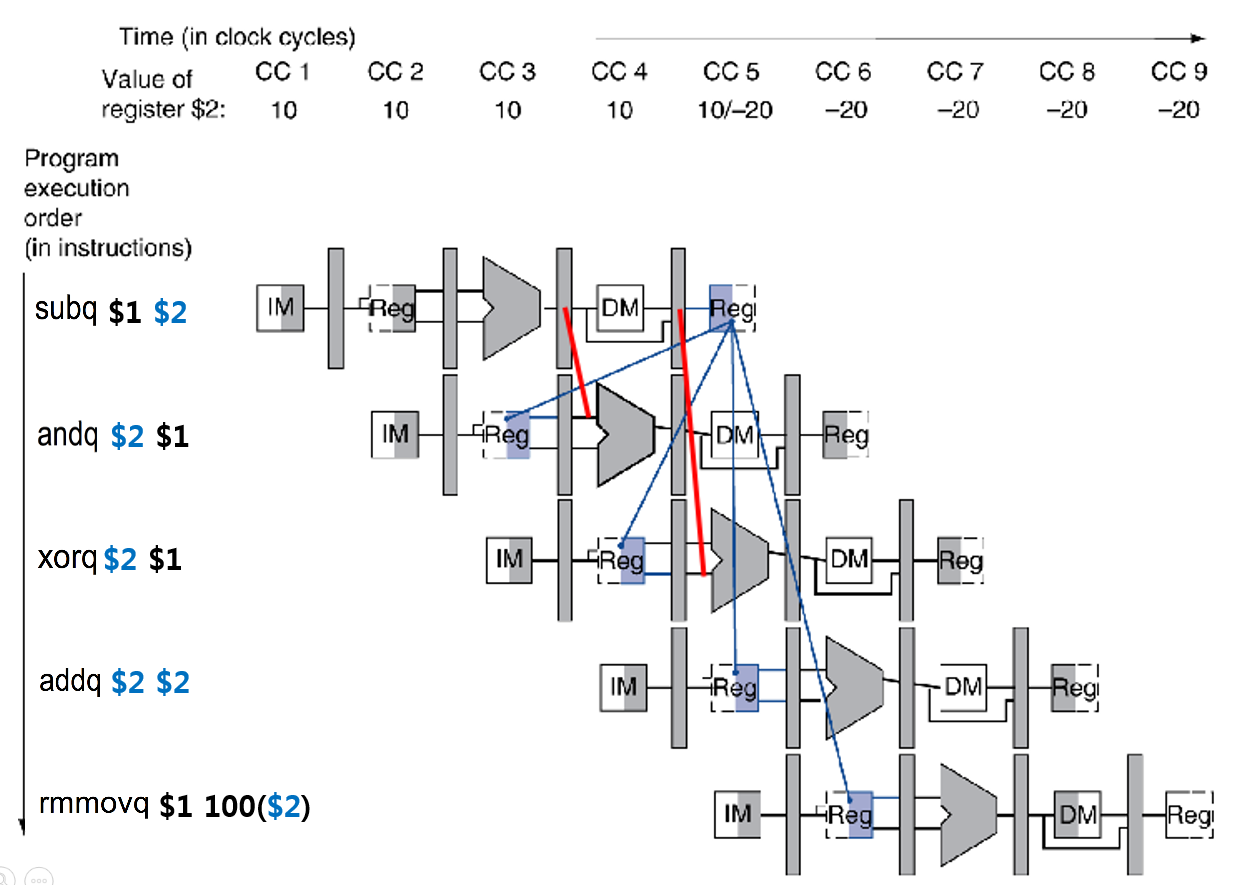
\includegraphics[scale=0.4]{forwarding.png}
		\caption{Bypassing example}
		\label{fig:2pipe_proc}
	\end{center}
\end{figure}

\noindent \paragraph{\bf Exercise 2 (40 points) :} 
You have to implement 6-stage pipelined processor with \texttt{bypassing} method, not the \texttt{scoreboard}.
Make a 'Proc\_bp.bsv' file by copying the 'Proc.bsv' after you have implemented the 6-stage pipelined processor 
and then modify it for \texttt{Exercise 2}.
\\Thus, you must have two modified files after you have finished this lab, 'Proc.bsv' for \texttt{Exercise 1} 
and 'Proc\_bp.bsv' for \texttt{Exercise 2}.

\end{document}
